\section{Basic analysis of the data}

\subsection{Analyse of trend and seasonalities}

Looking at the plot of the time serie for the mean monthly air temperature in Recife below (\autoref{fig:data-time-series}), we directly notice a seasonality in the data. This was obviously expected as the temperatures fluctuate between seasons. However, this is not clear if there is any trend (\textit{there seems to be a decrease in the mean monthly temperature which is kind of unexpected considering the climate change taking place since the beginning of the industrial era}) nor an instability in the variance. In order to have a clearer view of these elements, we can decompose the time serie by performing a \textbf{classical decomposition}. This method assume that the seasonal component repeat from year to year which is kind of a reasonable assumption for air temperature data. Let $\set{X_t, t \in \Z}$ be our time serie, assuming an additive decomposition we can write,

\begin{equation}
	X_t = S_t + T_t + R_t
\end{equation}
with $S_t$, $T_t$ and $R_t$ respectively the seasonal, the trend-cycle and the remainder components.

\begin{figure}[H]
	\centering
	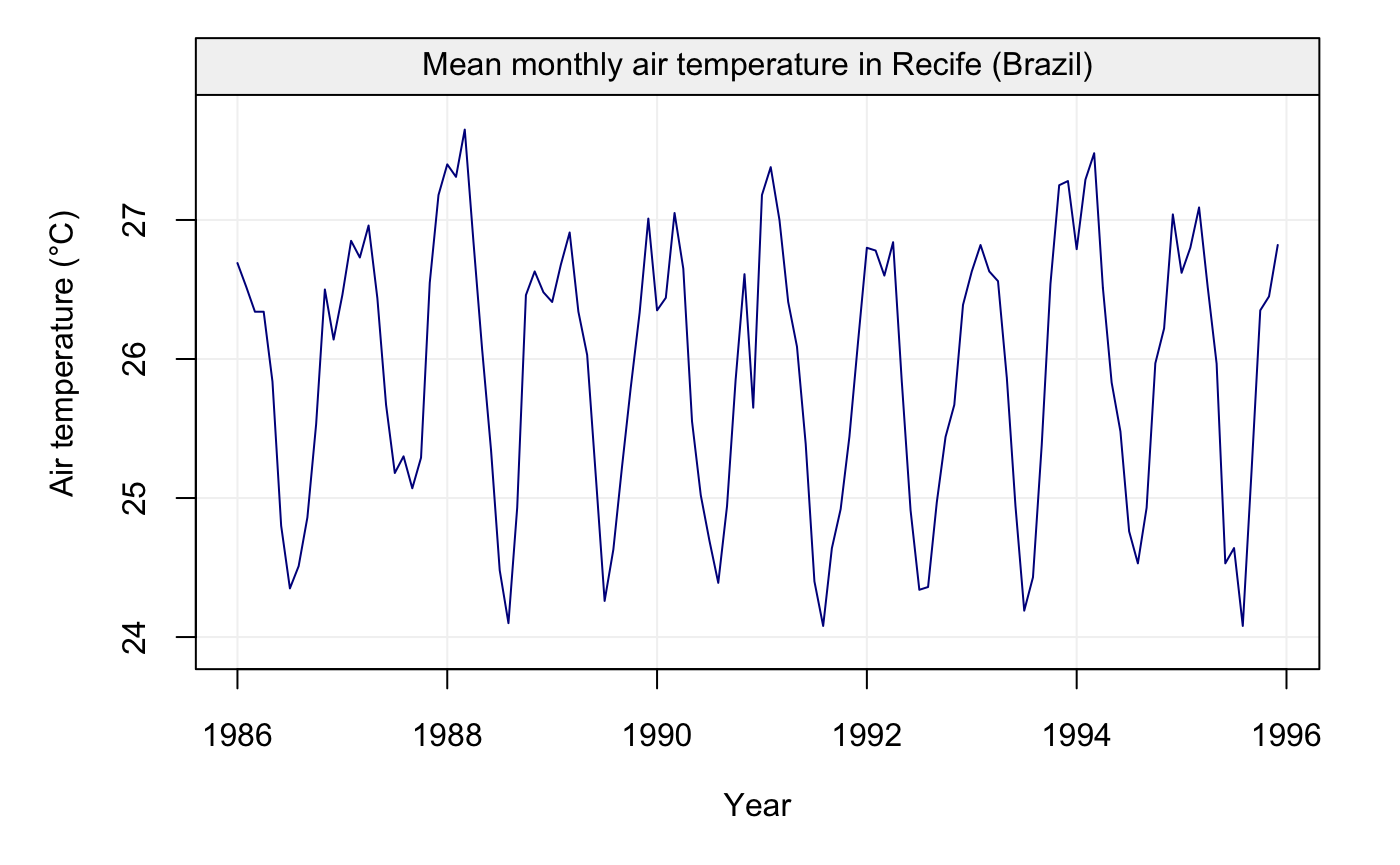
\includegraphics{figures/basic_analysis/data_time_series.png}
	\caption{Time series for the mean monthly air temperature in the city of Recife (Brazil) for the years $1986-1995$}
	\label{fig:data-time-series}
\end{figure}

\begin{figure}[H]
	\centering
	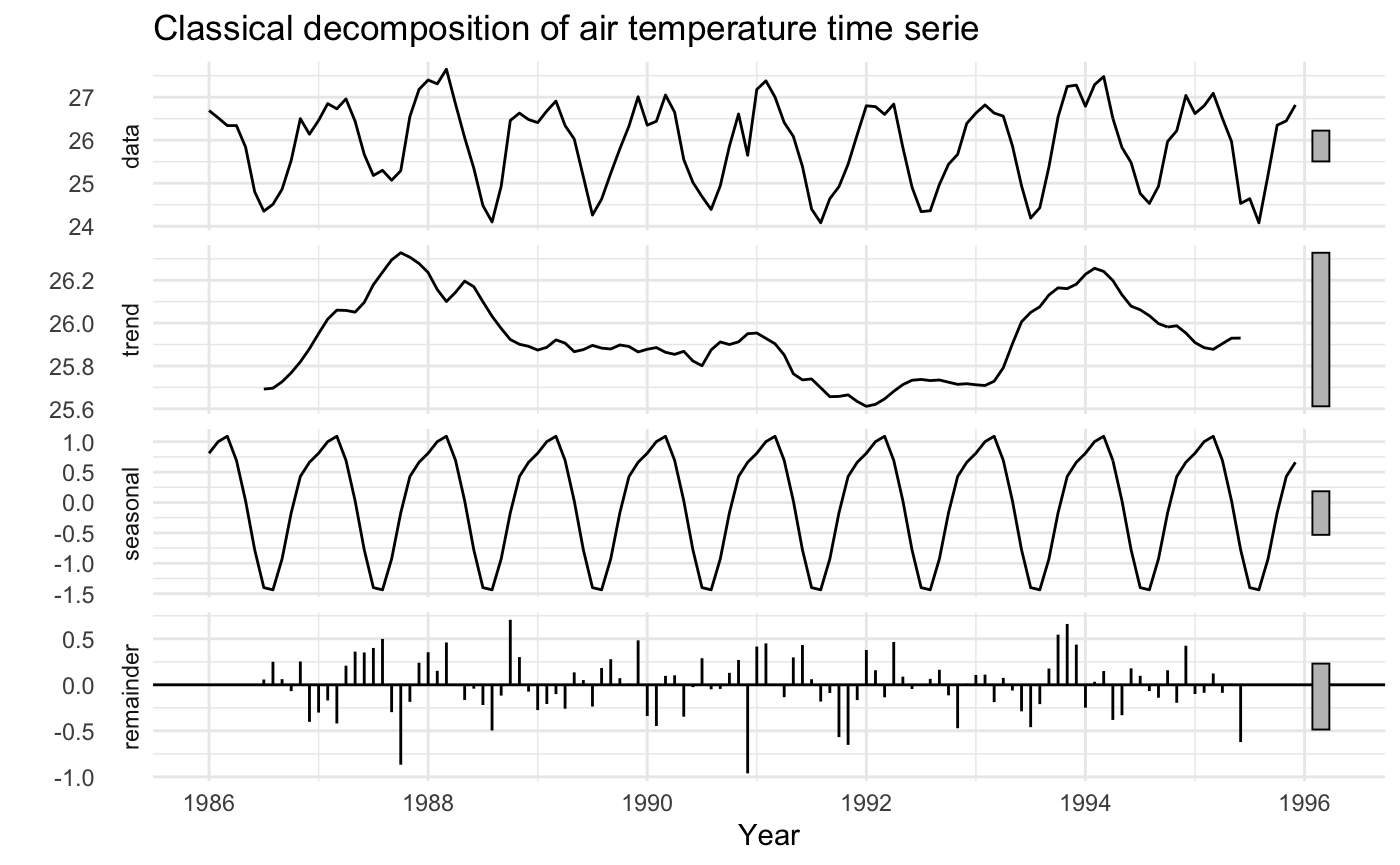
\includegraphics{figures/basic_analysis/time_serie_decomposition.png}
	\caption{Decomposition of the time serie $X_t$ into seasonal, trend-cycle and reminder components}
	\label{fig:data-classical-decomposition}
\end{figure}

Being situated in the southern hemisphere, the Brazil has its seasons inverted compared to our regions. 
This country is situated near the equator and therefore has pretty high temperature all the year long. However, the highest temperatures happen between the end and the beginning of the year and the lowest toward the middle of the year. That's clearly what we can notice in the seasonal part (\autoref{fig:data-classical-decomposition}). We can also notice a decreasing trend in the temperatures between $1988$ and $1993$ before it rises up again.